\documentclass[pdf]{beamer}

%\usepackage{lmodern}
\usepackage[font=scriptsize,skip=0pt,justification=justified,singlelinecheck=false]{caption}
%\usepackage{enumitem}
\usepackage{natbib}
\usepackage{bm}
\usepackage{mathtools}
\usepackage[makeroom]{cancel}

% Using underline
\usepackage{soul}

% =======================================
%   Using symbols for a checklist
% =======================================
\usepackage{pifont}% http://ctan.org/pkg/pifont
\newcommand{\cmark}{\ding{51}}%
\newcommand{\xmark}{\ding{55}}%

\usepackage{algorithm}
\usepackage{algpseudocode}
\usepackage{tikz}

\usepackage{amsmath}
\DeclareMathOperator*{\argmax}{arg\,max}
\DeclareMathOperator*{\argmin}{arg\,min}


%\usepackage[ruled,vlined]{algorithm2e}
%\usepackage{clrscode3e}

% ======================
%  Put Code into a Box
% ======================
%\usepackage{minted}
%\usepackage{tcolorbox}
%\usepackage{etoolbox}
%\BeforeBeginEnvironment{minted}{\begin{tcolorbox}}%
%\AfterEndEnvironment{minted}{\end{tcolorbox}}%



%\usepackage{adjustbox}

%remove the icon
\setbeamertemplate{bibliography item}{}

%remove line breaks
\setbeamertemplate{bibliography entry title}{}
\setbeamertemplate{bibliography entry location}{}
\setbeamertemplate{bibliography entry note}{}

% ======================================
%     Use number for caption
% ======================================
% \setbeamertemplate{caption}[numbered]{}

% ======================================
%     No Figure in the caption
% ======================================
%\setbeamertemplate{caption}{\insertcaption} ---> does not work
\captionsetup{labelformat=empty,labelsep=none} % ---> it works


\newtheorem{mydef}[theorem]{\Large \underline{\textbf{Definisi}}}

\makeatletter
\def\th@mystyle{%
    \normalfont % body font
    \setbeamercolor{block title example}{bg=blue,fg=white}
    \setbeamercolor{block body example}{bg=blue!20,fg=black}
    \def\inserttheoremblockenv{exampleblock}
  }
\makeatother
\theoremstyle{mystyle}
\newtheorem*{remark}{\textbf{Definition}}


% This file is a solution template for:

% - Talk at a conference/colloquium.
% - Talk length is about 20min.
% - Style is ornate.

% Copyright 2004 by Till Tantau <tantau@users.sourceforge.net>.
%
% In principle, this file can be redistributed and/or modified under
% the terms of the GNU Public License, version 2.
%
% However, this file is supposed to be a template to be modified
% for your own needs. For this reason, if you use this file as a
% template and not specifically distribute it as part of a another
% package/program, I grant the extra permission to freely copy and
% modify this file as you see fit and even to delete this copyright
% notice.  


\mode<presentation>
{
%  \usetheme{AnnArbor} % 
%	\usetheme{Frankfurt}
   \usetheme{Madrid}
  % or ...

%  \setbeamercovered{transparent}
  % or whatever (possibly just delete it)
}


\usepackage[english]{babel}
% or whatever

\usepackage[latin1]{inputenc}
% or whatever

\usepackage{times}
\usepackage[T1]{fontenc}
\usepackage{wasysym}

\usepackage{graphicx} % Necessary to use \scalebox

% Define absolute and norm
\DeclarePairedDelimiter\abs{\lvert}{\rvert}%
\DeclarePairedDelimiter\norm{\lVert}{\rVert}%

% ==============================
%       Redefine emphasize
% ==============================
\let\emph\relax % there's no \RedeclareTextFontCommand
\DeclareTextFontCommand{\emph}{\bfseries\em}


% Swap the definition of \abs* and \norm*, so that \abs
% and \norm resizes the size of the brackets, and the 
% starred version does not.
\makeatletter
\let\oldabs\abs
\def\abs{\@ifstar{\oldabs}{\oldabs*}}
%
\let\oldnorm\norm
\def\norm{\@ifstar{\oldnorm}{\oldnorm*}}
\makeatother

\usepackage{color}
\definecolor{myblue}{rgb}{.8,.8,1}
\usepackage{empheq}
% Or whatever. Note that the encoding and the font should match. If T1
% does not look nice, try deleting the line with the fontenc.

\newlength\mytemplen
\newsavebox\mytempbox

\makeatletter
\newcommand\mybluebox{%
    \@ifnextchar[%]
       {\@mybluebox}%
       {\@mybluebox[0pt]}}

\def\@mybluebox[#1]{%
    \@ifnextchar[%]
       {\@@mybluebox[#1]}%
       {\@@mybluebox[#1][0pt]}}

\def\@@mybluebox[#1][#2]#3{
    \sbox\mytempbox{#3}%
    \mytemplen\ht\mytempbox
    \advance\mytemplen #1\relax
    \ht\mytempbox\mytemplen
    \mytemplen\dp\mytempbox
    \advance\mytemplen #2\relax
    \dp\mytempbox\mytemplen
    \colorbox{myblue}{\hspace{1em}\usebox{\mytempbox}\hspace{1em}}}

\makeatother

\title[Interpretable ML] % (optional, use only with long paper titles)
{\textbf{Interpretable Machine Learning}}

\subtitle
{\textit{The Basics}}

\author[Hendra Bunyamin] % (optional, use only with lots of authors)
{Hendra Bunyamin}
%{F.~Author\inst{1} \and S.~Another\inst{2}} --> original
% - Give the names in the same order as the appear in the paper.
% - Use the \inst{?} command only if the authors have different
%   affiliation.

\institute[ ] % (optional, but mostly needed)
{
%  \inst{1}%
  Informatics Engineering\\
  Faculty of Information Technology\\
  Maranatha Christian University
%  \and
%  \inst{2}%
%  Department of Theoretical Philosophy\\
%  University of Elsewhere
}
% - Use the \inst command only if there are several affiliations.
% - Keep it simple, no one is interested in your street address.

\date[NUNI IT Online] % (optional, should be abbreviation of conference name)
{9 April 2021 \\ NUNI IT Online Seminar}
% - Either use conference name or its abbreviation.
% - Not really informative to the audience, more for people (including
%   yourself) who are reading the slides online

\subject{NUNI IT Online Seminar: AI}
% This is only inserted into the PDF information catalog. Can be left
% out. 

% If you have a file called "university-logo-filename.xxx", where xxx
% is a graphic format that can be processed by latex or pdflatex,
% resp., then you can add a logo as follows:

\pgfdeclareimage[height=1.5cm]{university-logo}{images/logo-mcu}
\logo{\pgfuseimage{university-logo}}


% Delete this, if you do not want the table of contents to pop up at
% the beginning of each subsection:
\AtBeginSection[]
{
  \begin{frame}<beamer>{Outline}
    \tableofcontents[currentsection,currentsection]
  \end{frame}
}


% If you wish to uncover everything in a step-wise fashion, uncomment
% the following command: 

%\beamerdefaultoverlayspecification{<+->}

\begin{document}

\begin{frame}
  \titlepage
\end{frame}

\begin{frame}{Outline}
  \tableofcontents
  % You might wish to add the option [pausesections]
\end{frame}


% Structuring a talk is a difficult task and the following structure
% may not be suitable. Here are some rules that apply for this
% solution: 

% - Exactly two or three sections (other than the summary).
% - At *most* three subsections per section.
% - Talk about 30s to 2min per frame. So there should be between about
%   15 and 30 frames, all told.

% - A conference audience is likely to know very little of what you
%   are going to talk about. So *simplify*!
% - In a 20min talk, getting the main ideas across is hard
%   enough. Leave out details, even if it means being less precise than
%   you think necessary.
% - If you omit details that are vital to the proof/implementation,
%   just say so once. Everybody will be happy with that.

%\begin{frame}{Make Titles Informative. Use Uppercase Letters.}{Subtitles are optional.}

\section{Introduction}
\begin{frame}{Introduction}
	\begin{figure}[!ht]
		\centering
		\includegraphics<2->[scale=.225]{images/AI-value-creation}
		\caption{\only<2->{Source: McKinsey Global Institute~\citep{ng2019AIForEveryone}}}
		\label{fig:ai-value-creation}
	\end{figure}
	\onslide<3-> \$$13$ trillion = \$$13 \times 10^{12} = \text{Rp}183.000.000.000.000.000,-$ 
\end{frame}

\begin{frame}{Demystifying AI}
	 Artificial Intelligence or \textbf{AI} can be divided into 2 as follows~\citep{ng2019AIForEveryone}:
	\begin{itemize}
		\item<2-> \textbf{ANI} $\Rightarrow$ Artificial Narrow Intelligence. \\
		\onslide<3-> Examples: smart speaker, self-driving car, web search, AI in farming and factories.
		\bigskip
		\item<4-> \textbf{AGI} $\Rightarrow$ Artificial General Intelligence. \\
		\onslide<5->Examples: Do anything a human can do or even more than human capability.
	\end{itemize}
	\begin{center}
		\includegraphics<6->[scale=.12]{images/ex-machina} \qquad \includegraphics<7->[scale=.12]{images/upgrade}
	\end{center}	
\end{frame}

\section{Machine Learning}
\begin{frame}{Diagram Venn tentang AI, ML, DL, Data Science}
	\begin{figure}[!ht]
		\centering
		\includegraphics<2->[scale=.45]{images/diagram-venn-deep-learning}
		\caption{\only<2->{Relationship among AI, ML, DL, and DS~\citep{kharkovyna2019ABeginnersGuide}}}
	\end{figure}
\end{frame}

\begin{frame}{Machine Learning}
	\begin{itemize}
		\item<2-> One of the tools that drive the significant progress of AI is \textbf{Machine Learning} (ML).
		\item<3-> \textbf{Machine Learning} is a set of methods that allow computers to \textit{learn from data} to \textit{make and improve predictions}, e.g., cancer, weekly sales, credit default.  
		\begin{figure}[!ht]
			\centering
			\includegraphics<4->[scale=0.18]{images/programming-with-without-ml}
			\caption{\only<4->{A paradigm shift from "normal programming" to "indirect programming"}}
		\end{figure}
	\end{itemize}	
	
\end{frame}


\begin{frame}{Machine Learning: Supervised Learning (1/2)}
	\begin{itemize}		
		\item<2-> A common type of of \textbf{Machine Learning} is a type of AI that learns from $X$ to $Y$	or is often called \emph{Supervised Learning}.
		
		\bigskip
		
		\begin{center}
			
			\scalebox{2}{
				$X \longrightarrow Y$
			} \\	
			\scalebox{1}{
				\qquad input \qquad \; \; output
			}							
		\end{center}
		
		\item<3-> A \textbf{Machine Learning Model} is \textit{the learned program} that maps inputs into outputs/predictions.
		\item<4-> A \textbf{Machine Learning Algorithm} is \textit{the program} used to learn a ML model from data~\citep{molnar2019}.
	\end{itemize}	
\end{frame}


\begin{frame}{Machine Learning: Supervised Learning (2/2)}
	\begin{table}[!ht]
		\centering
		\begin{tabular}{ccc|l}
			\textbf{Input ($\bm{X}$)} &  & \textbf{Output ($\bm{Y}$)} & \textbf{ML Model} \\
			\hline
			\onslide<2->{email     & $\longrightarrow$  & spam? (0/1)                & spam filtering}   \\
			          &                    &                            &                  \\
			\onslide<3->{audio     & $\longrightarrow$  & text transcript            & speech recognition}      \\
			          &                    &                            &                  \\
			\onslide<4->{English   & $\longrightarrow$  & Indonesia                  & machine translation} \\
			          &                    &                            &                  \\
			\onslide<5->{ad, user info & $\longrightarrow$ & click? (0/1)            & online advertising} \\
			          &                    &                               &                  \\
			\onslide<6->{image, radar info & $\longrightarrow$ & position of other cars &  self-driving car} \\
			          &                    &                               &                  \\
			\onslide<7->{image of phone & $\longrightarrow$ & defect? (0/1)             & visual inspection} \\
			\hline           			             
		\end{tabular}
	\end{table}
\end{frame}

\begin{frame}{Why Now?}
	\begin{figure}[!ht]
		\centering
		\includegraphics<2->[scale=.25]{images/big-data}
		\caption{\only<3->{Large neural net + Big Data = High Performance~\citep{ng2019AIForEveryone}}}
		\label{fig:big-data}
	\end{figure}
\end{frame}

\begin{frame}{Common Machine Learning Components}
Typically, a Machine Learning Algorithm consists of 

\bigskip
\begin{enumerate}
	\item<2-> Data $\rightarrow X = \left\{ x^{(1)}, x^{(2)}, \ldots, x^{(m)} \right\}$ dan $Y = \left\{ y^{(1)}, y^{(2)}, \ldots, y^{(m)} \right\}$

	\bigskip
	\item<3-> Model/Hypothesis $\rightarrow h$
	
	\bigskip  
	\item<4-> Cost/Loss Function $\rightarrow J$
	
	\bigskip
	\item<5-> Optimization Algorithm $\rightarrow$ \textit{gradient descent}
\end{enumerate}	

\bigskip
\onslide<6-> Let's walk through all these components in a concrete example!
\end{frame}

\section{Example: Predicting Profits of Food Trucks}
\begin{frame}{Predicting Profits for Food Trucks}
\onslide<2->Suppose you are the \textit{CEO of a restaurant franchise} and are considering different cities for opening a new outlet. \\ 
\onslide<3-> The franchise already \textit{has trucks in various cities} and you have \textit{data for profits and populations from the cities}.
	\begin{figure}[!ht]
		\centering
		\includegraphics<4->[scale=.05]{images/food-truck}
		\caption{\only<4->{A food truck serving chinese food\citep{louis2020foodtruck}}}
	\end{figure}	
\end{frame}


\section{A Machine Learning Component: Data}
\begin{frame}{Machine Learning Component: Data (1/2)}
\begin{table}[!ht]
	\centering
	\begin{tabular}{|c|r|}
		\hline
		\textbf{Population} ($\bm{X})$ & \multicolumn{1}{c|}{\textbf{Profit} ($\bm{Y}$)}  \\
		\hline
		6.1101 & 17.592 \\
		\hline
        5.5277 & 9.130 \\
        \hline
        8.5186 & 13.662 \\
        \hline
        \vdots & \vdots \\
        \hline
        5.4369 & 0.617 \\
        \hline		
	\end{tabular}
	\caption{\textbf{Population} of city is in 10,000s while \textbf{Profit} is in \$10,000s}	
\end{table} 
	\onslide<2-> We can write:
	\begin{align*}
		\onslide<3->{x_1^{(1)} = 6.1101 &\text{ and } y^{(1)} = 17.592} \\
		\onslide<4->{x_1^{(2)} = 5.5277 &\text{ and } y^{(2)} = 9.130} \\
		\onslide<5->{x_1^{(3)} = 8.5186 &\text{ and } y^{(3)} = 13.662, \text{ and}} \\
		\onslide<6->{x_1^{(97)} = 5.4369 &\text{ and } y^{(97)} = 0.617}				                 
	\end{align*}
\end{frame}

\begin{frame}{Machine Learning Component: Data (2/2)}
 	\begin{figure}[!ht]
 		\centering
 		\includegraphics<2->[scale=.2]{images/scatter-plot-food-truck}
 		\caption{\only<2->{Scatter plot of food trucks data}}
 	\end{figure}
\end{frame}

\section{A Machine Learning Component: Model/Hypothesis}
\begin{frame}{Machine Learning Component: Model (1/3)}
	\onslide<2-> We utilize a linear regression model as our model/hypothesis:
	\begin{align*}
		\onslide<3->{h_{\theta}(x) &= \theta_0 + \theta_1 x_1} \\
		             \onslide<4->{&= \begin{bmatrix}
		     1 & x_1         
\end{bmatrix}	\begin{bmatrix}
	\theta_0 \\
	\theta_1
\end{bmatrix}} 	                	\\
                  \onslide<5->{  &= x \theta}
	\end{align*}
	\onslide<6-> Since we have $97$ instances, we write $X$ as 
\begin{equation*}
	\onslide<7->{X = \begin{bmatrix}
		1      & x_1^{(1)} \\ 
		1      & x_1^{(2)} \\
		\vdots & \vdots \\
		1      & x_1^{(97)}
	\end{bmatrix},} 
\end{equation*}
\onslide<8-> $X$ is also called a \textit{design matrix}.
\end{frame}

\begin{frame}{Machine Learning Component: Model (2/3)}
therefore, we can construct our model for each instance as follows:
\begin{align*}
	\onslide<2->{\begin{bmatrix}
		h_{\theta}(x^{(1)}) \\
		h_{\theta}(x^{(2)}) \\
		\vdots \\
		h_{\theta}(x^{(97)})				
	\end{bmatrix} &=} \onslide<3->{\begin{bmatrix}
		1      & x_1^{(1)} \\ 
		1      & x_1^{(2)} \\
		\vdots & \vdots \\
		1      & x_1^{97}
	\end{bmatrix} \begin{bmatrix}
		\theta_0 \\
		\theta_1
	\end{bmatrix}}  \\
	\onslide<4->{&= X \theta}
\end{align*}
\onslide<5->$X \theta$ is our \textit{vectorized hyphotesis/model}.

\bigskip
\onslide<6->Utilizing a product of two matrices $\Longrightarrow$ improve computing efficiency.
\end{frame}

\begin{frame}{Machine Learning Component: Model (3/3)}
	Assuming that we have $\theta$, we can compute and plot our regression line as follows:
	\begin{figure}[!ht]
		\centering
		\includegraphics<2->[scale=.2]{images/linear-regression-food-truck}
		\caption{\only<3->{The regression line; however, how do we find $\theta_0$ and $\theta_1$?}}
		\label{fig:linear-regression-food-truck}
	\end{figure}
\end{frame}


%\begin{frame}{Machine Learning Component: Data (1/3)}
%	\begin{table}[!ht]
%		\centering
%		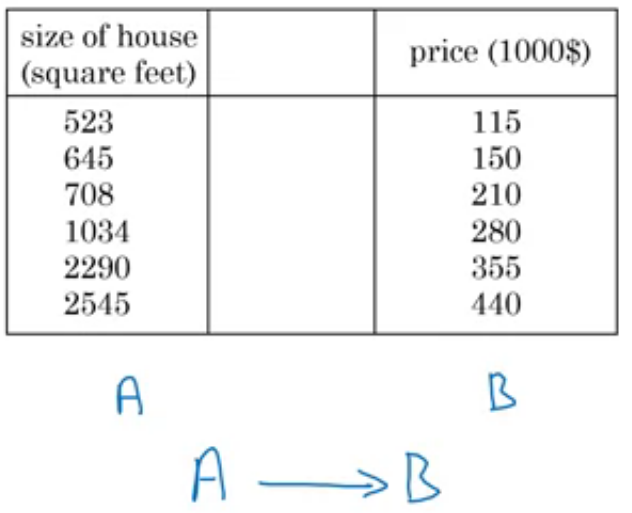
\includegraphics[scale=.3]{images/example-dataset-2}
%		\caption{House prices dataset~\citep{ng2019AIForEveryone}}
%		\label{fig:example-dataset-2}
%	\end{table}
%\end{frame}


%\begin{frame}{Example of a Table of Data (Dataset) (2/3)}
%	\begin{table}[!ht]
%		\centering
%		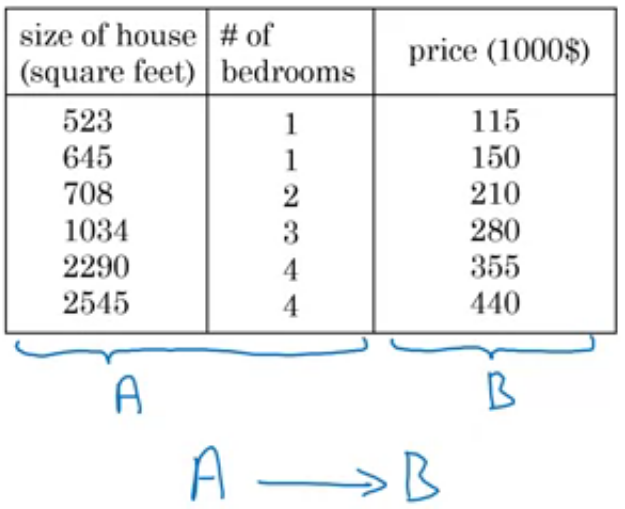
\includegraphics[scale=.3]{images/example-dataset-1}
%		\caption{House prices dataset~\citep{ng2019AIForEveryone}}
%		\label{fig:example-dataset-1}
%	\end{table}
%\end{frame}
%
%\begin{frame}{Example of a Table of Data (Dataset) (3/3)}
%	\begin{table}[!ht]
%		\centering
%		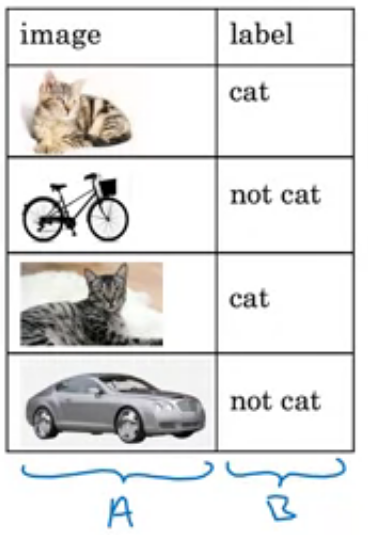
\includegraphics[scale=.3]{images/example-dataset-3}
%		\caption{Cat images dataset~\citep{ng2019AIForEveryone}}
%		\label{fig:example-dataset-3}
%	\end{table}
%\end{frame}
%
%\begin{frame}{Acquiring data}
%	\begin{itemize}
%		\item Manual labeling
%		\begin{center}
%			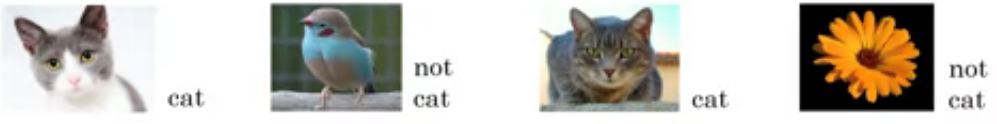
\includegraphics[scale=.3]{images/manual-labeling}
%		\end{center}
%		\item From observing behaviors
%		\begin{center}
%			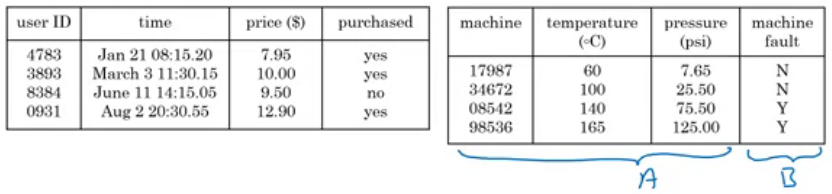
\includegraphics[scale=.35]{images/observing-behaviors}
%		\end{center}
%		\item Download from websites / partnerships		
%	\end{itemize}
%\end{frame}

%\begin{frame}{Data is Messy}
%	\begin{itemize}
%		\item Garbage in, garbage out
%		\item Data problems: \textit{incorrect labels} and \textit{missing values} 
%		\begin{center}
%			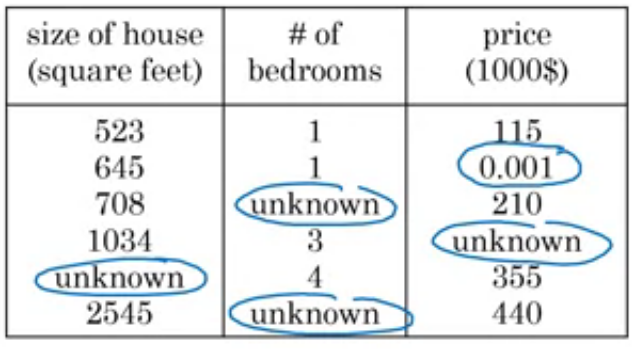
\includegraphics[scale=.3]{images/data-problems} 
%		\end{center}
%		\item Multiple types of data \\
%		\textit{images}, \textit{audio}, \textit{text} $\Rightarrow$ \textbf{unstructured data}					
%	\end{itemize}
%\end{frame}
%

\section{A Machine Learning Component: Cost/Lost Function}
\begin{frame}{Machine Learning Component: Cost Function (1/3)}
A Cost/Loss Function calculates \textit{all the errors made by the model}.

\begin{figure}[!ht]
	\centering
	\includegraphics<2->[scale=.16]{images/example-of-errors}
	\caption{\only<2->{\textit{An example of errors}; Specifically \textit{the black lines} represent the error associated with each instance~\citep{james2013introduction}}}
\end{figure}
\end{frame}

\begin{frame}{Machine Learning Component: Cost Function (2/3)}
The Cost/Loss Function is usually denoted as $J$; moreover, in case of linear regression:
\begin{align*}
	J(\theta) &= \onslide<3->{\frac{1}{2m}} \onslide<2->{\sum_{i=1}^{m}{\left(h_{\theta}(x^{(i)}) - y^{(i)}\right)^2}} \\
	          &= \onslide<4->{\frac{1}{2 \times 97} \sum_{i=1}^{97}{\left(h_{\theta}(x^{(i)}) - y^{(i)}\right)^2}}  \\
	          &= \onslide<5->{\frac{1}{2 \times 97} \sum_{i=1}^{97}{\left(\theta_0 + \theta_1 x_1^{(i)} - y^{(i)}\right)^2}}
\end{align*}
\onslide<6->\textbf{The Goal}: \onslide<7->How do we minimize \textbf{the cost function}? 
\begin{block}{}
\onslide<8-> We need \textbf{Calculus}.
\end{block}
\end{frame}

\begin{frame}{Machine Learning Component: Cost Function (3/3)}
	We need to find $\theta_0$ and $\theta_1$ which minimize $J(\theta)$, that is
	\begin{equation*}
		\argmin_{\theta_0, \theta_1}{ \onslide<2->{\left\{  \frac{1}{2 \times 97} \sum_{i=1}^{97}{\left(\theta_0 + \theta_1 x_1^{(i)} - y^{(i)}\right)^2} \right\}}}.
	\end{equation*}
\onslide<3->How do we find $\theta_0$ and $\theta_1$ that minimize the \textbf{cost function}?
\begin{block}{}
\onslide<4-> We need an \textbf{Optimization Algorithm}.
\end{block}	
\end{frame}

\section{A Machine Learning Component: Optimization Algorithm}
\begin{frame}{ML Component: Optimization Algorithm (1/7)}
	A famous optimization algorithm: \onslide<2-> \textbf{Gradient Descent}
	\begin{figure}[!ht]
		\centering
		\includegraphics<3->[scale=.175]{images/gradient-descent-works}
		\caption{\only<3->{Gradient descent in action~\citep{geron2019handson}}}
		\label{fig:gradient-descent-works}
	\end{figure}	
\end{frame}

\begin{frame}{ML Component: Optimization Algorithm (2/7)}
	\textbf{Gradient Descent} is a simple algorithm:
	\begin{equation*}
		\onslide<2->{\theta_{\text{new}} = \theta_{\text{old}} - \alpha \times \frac{\partial{J}}{\partial{\theta}}}
	\end{equation*}
	\onslide<3->with $\alpha$ is a \textit{learning rate} and $\frac{\partial{J}}{\partial{\theta}}$ is called the \textit{gradient}. 
	
	\bigskip
	\onslide<4-> The \textit{gradient} is the \textbf{partial derivative} of $J$\\ 
	(We need \textbf{Calculus} to calculate this one).
\end{frame}

\begin{frame}{ML Component: Optimization Algorithm (3/7)}
Our cost/loss function for linear regression:
\begin{equation*}
	J(\theta) = \frac{1}{2 \times 97} \times \sum_{i=1}^{97}{\left(\theta_0 + \theta_1 x_1^{(i)} - y^{(i)}\right)^2}
\end{equation*}	

With the help of \textbf{Calculus}, we have

\begin{align*}
	\frac{\partial{J}}{\partial{\theta_0}} &= \onslide<2->{ \left( \frac{1}{97 \times 2} \right)} \onslide<3->{\times  2} \onslide<4->{\times \sum_{i=1}^{97}{\left(\theta_0 + \theta_1 x_1^{(i)} - y^{(i)}\right)} }  \\
	                                       &= \onslide<5->{\left( \frac{1}{97 \times \cancel{2}} \right) \cancel{2} \times \sum_{i=1}^{97}{\left(\theta_0 + \theta_1 x_1^{(i)} - y^{(i)}\right)} }  \\
	                                       &= \onslide<6->{\frac{1}{97} \sum_{i=1}^{97}{\left(\theta_0 + \theta_1 x_1^{(i)} - y^{(i)}\right) }.}
\end{align*}
\end{frame}

\begin{frame}{ML Component: Optimization Algorithm (4/7)}
Our cost/loss function for linear regression:
\begin{equation*}
	J(\theta) = \frac{1}{2 \times 97} \times \sum_{i=1}^{97}{\left(\theta_0 + \theta_1 x_1^{(i)} - y^{(i)}\right)^2}
\end{equation*}	

Again with the help of \textbf{Calculus}, we have

\begin{align*}
	\frac{\partial{J}}{\partial{\theta_1}} &= \onslide<2->{\left( \frac{1}{97 \times 2} \right)} \onslide<3->{\times 2} \onslide<4->{\times \sum_{i=1}^{97}{\left(\theta_0 + \theta_1 x_1^{(i)} - y^{(i)}\right)} \onslide<5->{x_1^{(i)} }}  \\
	                                       &= \onslide<6->{\left( \frac{1}{97 \times \cancel{2}} \right) \cancel{2} \times \sum_{i=1}^{97}{\left(\theta_0 + \theta_1 x_1^{(i)} - y^{(i)}\right) x_1^{(i)} }}  \\
	                                       &= \onslide<7->{\frac{1}{97} \sum_{i=1}^{97}{\left(\theta_0 + \theta_1 x_1^{(i)} - y^{(i)}\right) x_1^{(i)} }.}	 
\end{align*}
\end{frame}

\begin{frame}{ML Component: Optimization Algorithm (5/7)}
As a summary, we have

\begin{align*}
	\onslide<2->{\theta_0 = \theta_0 - \alpha \times \frac{1}{97} \sum_{i=1}^{97}{\left(\theta_0 + \theta_1 x_1^{(i)} - y^{(i)}\right) } \text{ and}} \\
	\onslide<3->{\theta_1 = \theta_1 - \alpha \times \frac{1}{97} \sum_{i=1}^{97}{\left(\theta_0 + \theta_1 x_1^{(i)} - y^{(i)}\right) x_1^{(i)} }	}
\end{align*}
\end{frame}

\begin{frame}{ML Component: Optimization Algorithm (6/7)}
\textit{Learning rate} ($\alpha$) is the size of the steps.

\begin{figure}[!ht]
	\centering
	\includegraphics<2->[scale=.2]{images/learning-rate-too-small}
	\caption{\only<2->{This will happen when the $\alpha$ is too small~\citep{geron2019handson}}}
	\label{fig:learning-rate-too-small}
\end{figure}

\end{frame}

\begin{frame}{ML Component: Optimization Algorithm (7/7)}
What happens when $\alpha$ is too large?
\begin{figure}[!ht]
	\centering
	\includegraphics<2->[scale=.2]{images/learning-rate-too-large}
	\caption{\only<2->{This will happen when $\alpha$ is too large~\citep{geron2019handson}}}
	\label{fig:learning-rate-too-large}
\end{figure}
\end{frame}

\section{Demo from Stanford Machine Learning}
\begin{frame}{Demo Time}
We show a \textit{Linear Regression} as our Machine Learning demo\footnote{https://www.coursera.org/learn/machine-learning}.
\end{frame}
	
\section{Interpretability}
\begin{frame}{Importance of Interpretability}
	Why?
	\begin{itemize}
		\item<2-> A \textit{single metric}, for example: \textit{classification accuracy}, is an \textit{incomplete description} of most real-world tasks.
		
		\bigskip		
		\item<3-> The '\textit{Why}' can help you learn more about \textit{the problem}, \textit{the data}, and \textit{the reason} why a model might fail. \\
		
		\bigskip
		\item<4-> \textit{Human curiosity} and \textit{learning} $\Longrightarrow$ \textit{interpretability} \& \textit{explanations}. 
	\end{itemize}
	\begin{block}<4->{}
	\onslide<5->That's why we need the \textbf{interpretability of machine learning}. 	
	\end{block}	
\end{frame}

\begin{frame}{When We Do NOT Need Interpretability}
	\begin{itemize}
		\item<2-> Interpretability is not required if the model has \textit{no significant impact}. \\
		\onslide<3->{\textbf{Example}: Predict where our friends will go for their next culinary tour based on Instagram/Facebook data.}
		
		\bigskip
		\item<4-> Interpretability is not required when \textit{the problem is well-studied}. \\ 
		\onslide<5->\textbf{Example}: A machine learning model for OCR that processes images from envelopes and extracts addresses.		
	\end{itemize}
\end{frame}

\begin{frame}{The Black Box of Machine Learning~\citep{manpreet2019deeplearning}}
	\begin{figure}[!ht]
		\centering
		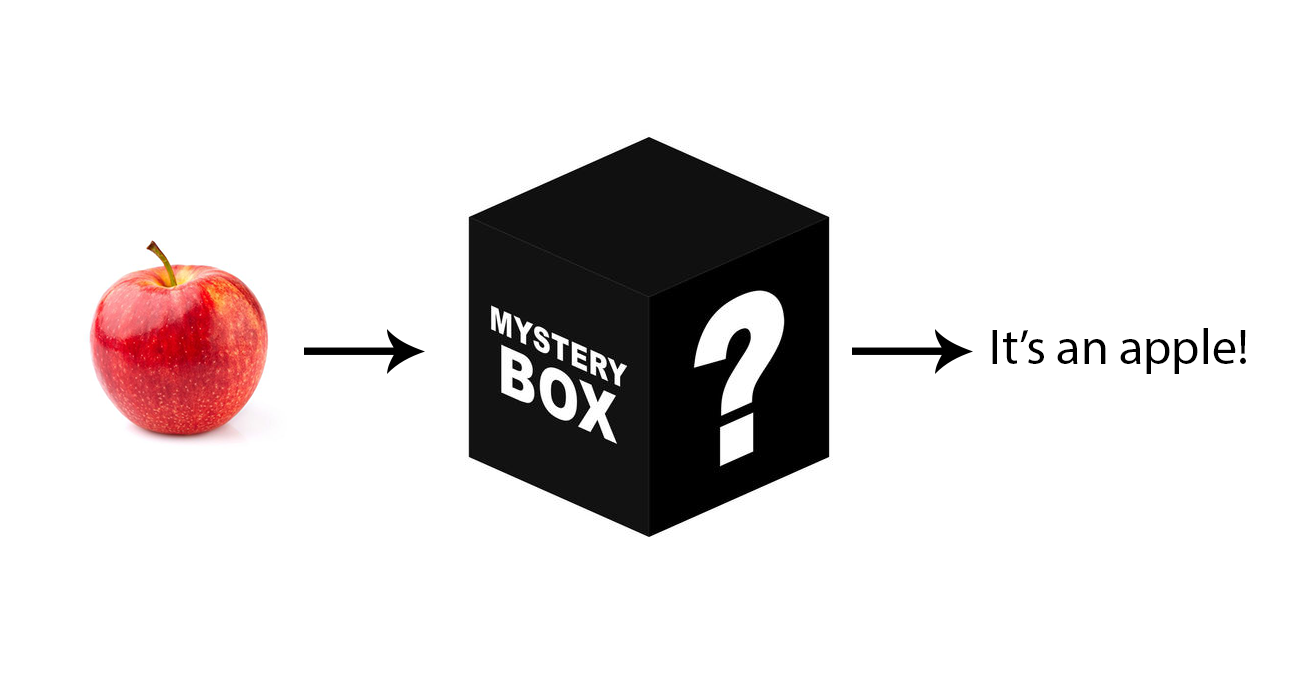
\includegraphics[scale=1]{images/deeplearningblackbox}
	\end{figure}	
\end{frame}

\begin{frame}{White Box vs Black Box~\citep{masis2021interpretable}}
	\begin{figure}[!ht]
		\centering
		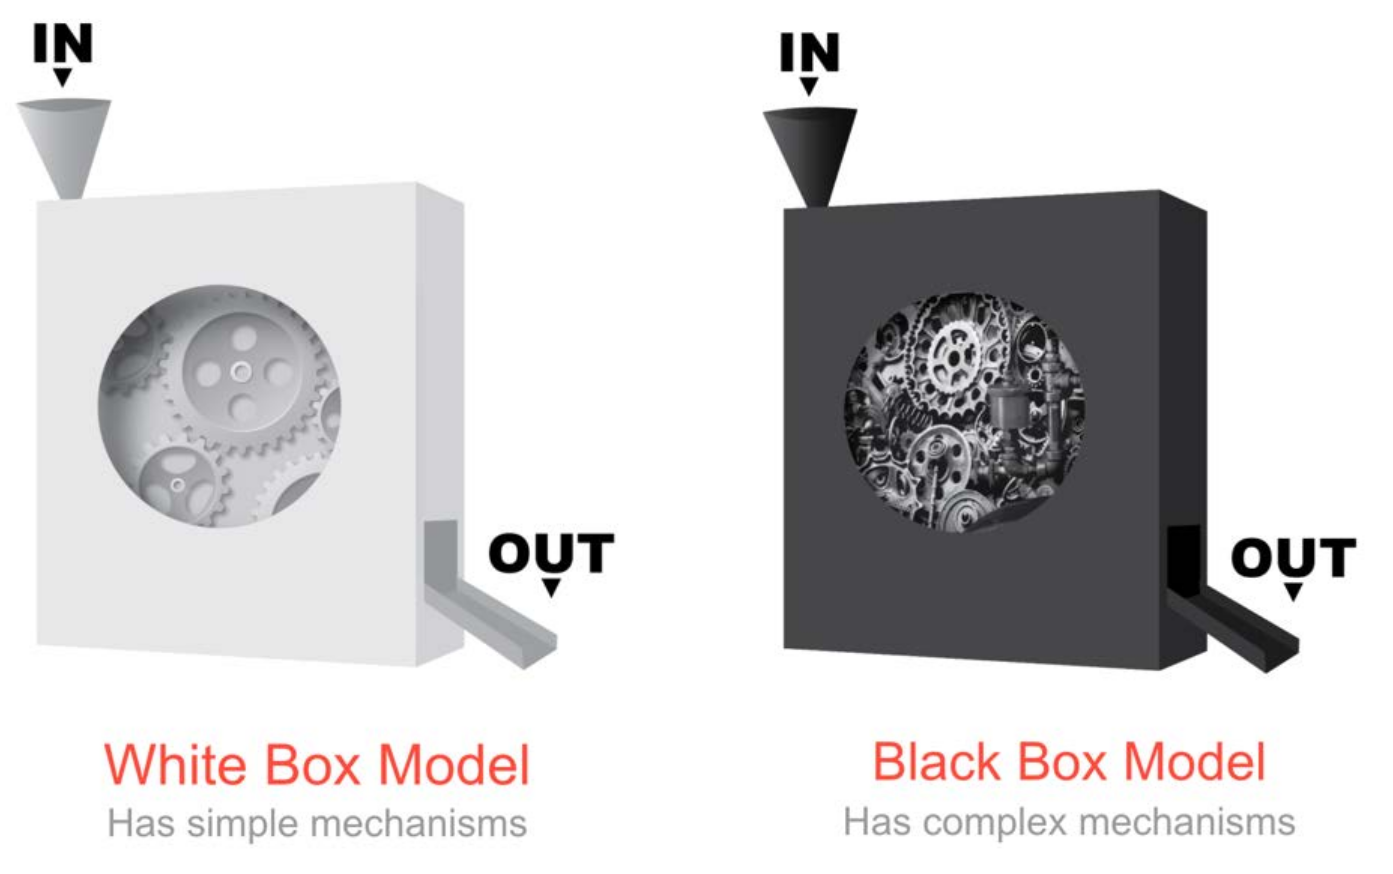
\includegraphics[scale=0.18]{images/white-box-and-black-box}
	\end{figure}
	\begin{block}{}
		\onslide<2->White box models are \textit{transparent}. \\
		\onslide<3->They achieve \textit{total} or \textit{near-total interpretation transparency} \\
		\onslide<4->$\Longrightarrow$ \textbf{interpretable}.
	\end{block}	 
\end{frame}

\section{Interpretable Models}
\begin{frame}{Interpretable Models (1/3)}
	\begin{itemize}
		\item The easiest way to achieve interpretability is \onslide<2->to \textit{use a subset of algorithms that create interpretable models}.
		
		\bigskip
		\item<3-> Commonly used interpretable models~\citep{molnar2019} are 
		\begin{itemize}
			\item<4-> \textbf{linear regression} $\Longrightarrow$ We'll talk about this later,
			\item<5-> logistic regression,
			\item<6-> other linear regression extensions, such as \textit{Generalized Linear Models} (GLMs) and \textit{Generalized Additive Models} (GAMs), 
			\item<7-> decision tree,
			\item<8-> decision rules, and
			\item<9-> the RuleFit algorithm.
		\end{itemize}
	\end{itemize}

	\begin{figure}[!ht]
		\centering
		\includegraphics<7->[scale=.3]{images/decision-tree}
		\caption{\only<7->{An example of a decision tree~\citep{chavan2019acomprehensive}}}
	\end{figure}	
\end{frame}

\begin{frame}{Interpretable Models (2/3)}
	The properties of interpretable models:
	\begin{itemize}
		\item<2-> A model is \textbf{linear} if the association between features and target is modelled linearly. 
		\item<3-> A model with \textbf{monotonicity constraints} ensures that the relationship between a feature and the target outcome always goes in the same direction over the entire range of the feature \\
		$\Longrightarrow$ easier to understand a relationship.
		\item<4-> Some models can automatically include \textbf{interactions between features} to predict the target outcome \\
		$\Longrightarrow$ improve predictive performance. \\
		\onslide<5->A famous example comes from \citet{james2013introduction}.
	\end{itemize}
\end{frame}

\begin{frame}{Interpretable Models (3/3)}
	\begin{table}[!ht]
		\centering
		\begin{tabular}{|l|c|c|c|l|}
			\hline
			\multicolumn{1}{|c|}{\textbf{Algorithm}} & \multicolumn{1}{c|}{\textbf{Linear}} & \multicolumn{1}{c|}{\textbf{Monotone}} & \multicolumn{1}{c|}{\textbf{Interaction}} & \multicolumn{1}{c|}{\textbf{Task}} \\
			\hline
			\onslide<2->{Linear regression   & \cmark & \cmark & \xmark & regr} \\
			\hline 
			\onslide<3->{Logistic regression & \xmark & \cmark & \xmark	 & class} \\
			\hline
			\onslide<4->{Decision trees      & \xmark & \textbf{?}      & \cmark & class, regr} \\
			\hline			
			\onslide<5->{RuleFit             & \cmark & \xmark & \cmark & class, regr} \\
			\hline
			\onslide<6->{Na\"{i}ve-Bayes     & \xmark & \cmark & \xmark & class} \\
			\hline
			\onslide<7->{$k$-nearest neighbors 	& \xmark & \xmark & \xmark & class, regr} \\
			\hline
		\end{tabular}
		\caption{\only<4->{\textbf{?} indicates that a decision tree can \textit{sometimes} be monotone}}
	\end{table}
	\onslide<8->We shall explore a \textbf{linear regression algorithm} as an example of \textit{interpretable model}. 	
\end{frame}

\section{Example of an Interpretable Model}
\begin{frame}{Example of Interpretable Model: Dataset (1/3)}
	\begin{itemize}
		\item<2-> Dataset: \textbf{Bike Rentals} (Regression).
		\item<3-> This dataset contains \textit{daily counts of rented bicycles} from the bicycle rental company Capital-Bikeshare\footnote{https://www.capitalbikeshare.com} in Washington D.C. 
		\item<4-> The goal is to \textit{predict how many bikes will be rented} depending on the weather and the day.
	\end{itemize}
\end{frame}

\begin{frame}{Example of an Interpretable Model: Dataset (2/3)}
	Here are the \textit{nine features} that are used:
	\begin{itemize}
		\item<2-> Count of bicycles \onslide<3->{$\Longrightarrow y$ }
		\item<4-> The season, either spring, summer, fall, or winter
		\item<5-> Indicator whether the day was a holiday or not
		\item<6-> Number of days since the 01.01.2011 (the first day in the dataset)
		\item<7-> Indicator whether the day was a working day or weekend
		\item<8-> The weather situation on that day: good, misty, or rain/snow/storm
		\item<9-> Temperature in degrees Celcius
		\item<10-> Relative humidity in percent (0 to 100)	
		\item<11-> Wind speed in km per hour	 
	\end{itemize}
\end{frame}

\begin{frame}{Example of Interpretable Model: Dataset (3/3)}
	\begin{figure}[!ht]
		\centering
		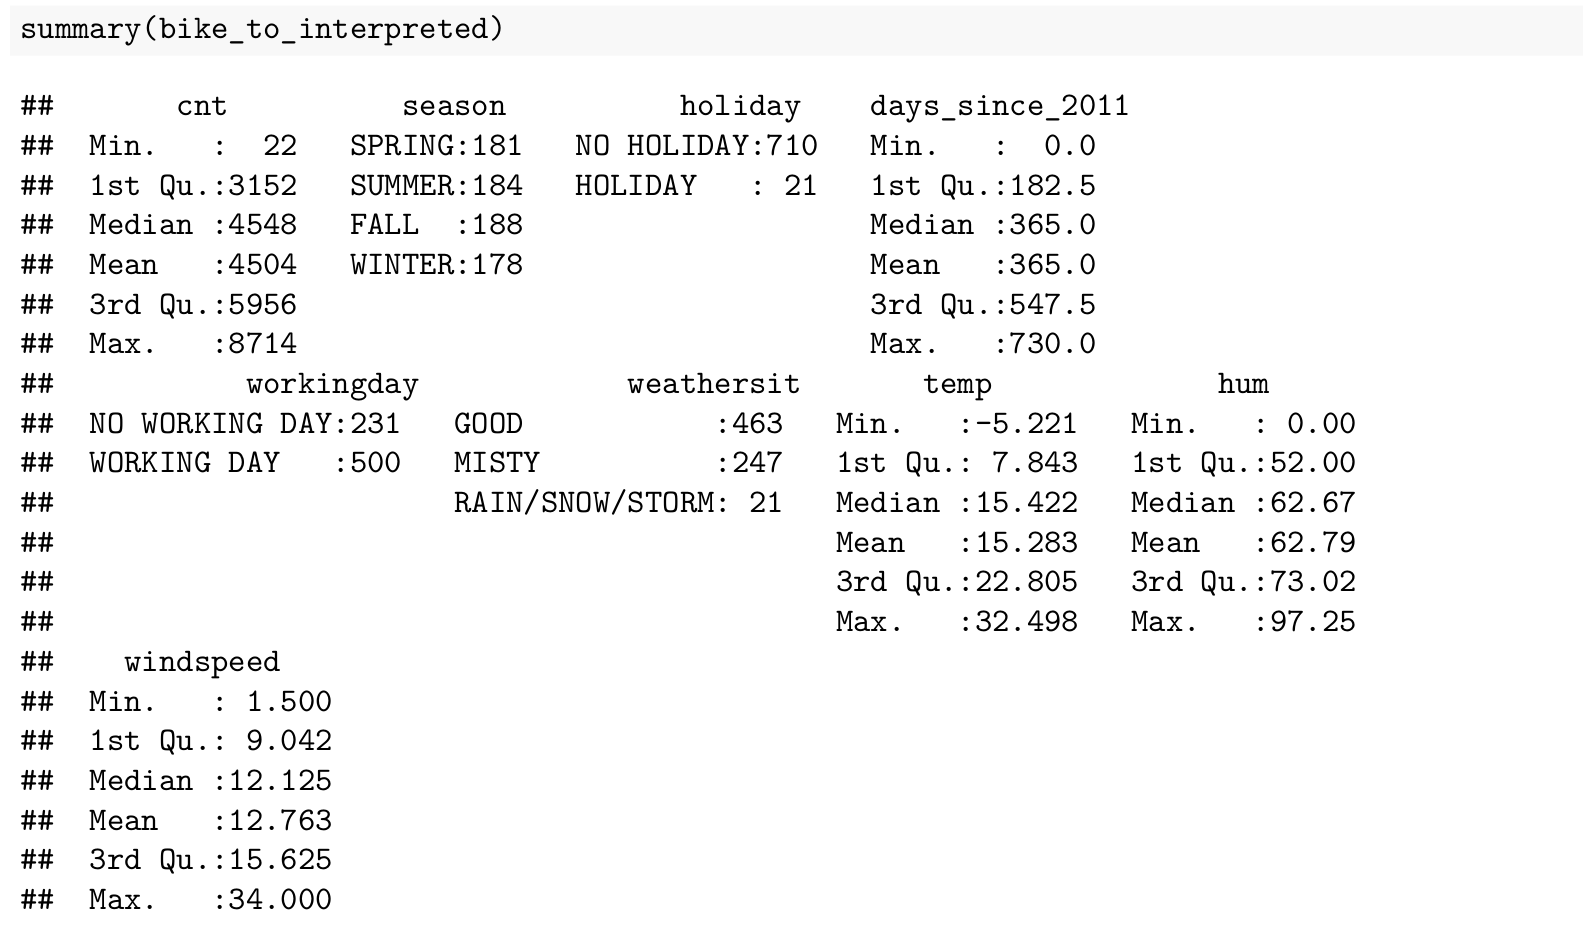
\includegraphics[scale=.21]{images/summary-bike}
		\caption{A summary of \texttt{bike\_to\_interpreted} dataset}
	\end{figure}
\end{frame}

\begin{frame}{Example of Interpretable Model: Linear Regression}
	The learned relationships between $X$ and $y$ are \textbf{linear} and can be written for a single instance $i$ as follows:
	\begin{equation*}
		\onslide<2->{y = \theta_0 + \theta_1 x_1 + \cdots + \theta_p x_p + \epsilon}
	\end{equation*}
	\onslide<3->{The epsilon ($\epsilon$) is the \textbf{error} we still make, i.e. the difference between the prediction and the actual outcome.}
\end{frame}

\begin{frame}{Linear Regression Assumptions}
	Whether the linear regression model is the "correct" model depends on whether the relationships in the data meet certain assumptions~\citep{kassambara2018linear}, which are
	\begin{itemize}
		\item<2-> \textbf{Linearity of the data} \onslide<3->{$\rightarrow$ the relationship between the predictor ($X$) and the outcome ($y$) is assumed to be linear.} 
		\item<4-> \textbf{Normality of residuals} \onslide<5->{$\rightarrow$ the residual errors are assumed to be \textit{normally distributed}.}
		\item<6-> \textbf{Homoscedasticity} \onslide<7->{$\rightarrow$ the residuals are assumed to have a \textit{constant variance}.}
		\item<8-> \textbf{Independence of residuals error terms} \onslide<9->{$\rightarrow$ each instance is \textit{independent} of any other instance.}
	\end{itemize}
\end{frame}

\section{Example: How to Interpret the Model}
\begin{frame}{Example of Interpretable Model: How to Interpret (1/5)}
	The linear regression model:
	\begin{equation*}
		y = \theta_0 + \theta_1 x_1 + \cdots + \theta_p x_p + \epsilon
	\end{equation*}

	\onslide<2->{The interpretation of the features in the linear regression model can be automated by using following text templates:}
	
	\bigskip
	\begin{itemize}
		\item<3-> \textbf{Interpretation of a Numerical Feature} \\
		\onslide<4->{An increase of feature $x_k$ by one unit increases the prediction for $y$ by $\theta_k$ units when \textit{all other feature values remain fixed}.} 
		
		\bigskip
		\item<5-> \textbf{Interpretation of a Categorical Feature} \\
		\onslide<6->Changing feature $x_k$ from the reference category to the other category increases the prediction for $y$ by $\theta_k$ when \textit{all other features remain fixed}.	
	\end{itemize}
\end{frame}


\begin{frame}{Example of Interpretable Model: How to Interpret (2/5)}
	\begin{itemize}
		\item<2-> Another important measurement for interpreting linear models is \onslide<3->{the $\bm{R}$\textbf{-squared} measurement.}
		
		\bigskip
		\item<4-> $\bm{R}$\textbf{-squared} tells us how much of the total variance of your target outcome is explained by the model. 
		
		\bigskip
		\item<5-> The higher $\bm{R}$\textbf{-squared}, the better our model explains the data.
	\end{itemize}
\end{frame}

\begin{frame}{Example of Interpretable Model: How to Interpret (3/5)}
		The formula for calculating $\bm{R}$\textbf{-squared} is:
		\begin{equation*}
			\onslide<2->{R^2 = \frac{1-SSE}{SST}}
		\end{equation*}
		\onslide<3->{with $SSE$ is squared sum of the error terms:}
		\begin{equation*}
			\onslide<4->{SSE = \sum_{i=1}^{m}{\left(h_{\theta}(x^{(i)}) - y^{(i)}\right)^2}}
		\end{equation*}
		\onslide<5->{and $SST$ is the squared sum of the data variance:}
		\begin{equation*}
			\onslide<6->{SST = \sum_{i=1}^{m}{(\overline{y} - y^{(i)})^2} \text{ with }\overline{y} = \frac{\sum_{i=1}^m{y^{(i)}}}{m}}
		\end{equation*}				
		\onslide<7->{$\bm{R}$\textbf{-squared} tells us how much of our variance can be explained \\ by the linear model ($0 \leq R\text{-squared} \leq 1$).}
\end{frame}

\begin{frame}{Example of Interpretable Model: How to Interpret (4/5)}
%	Since $\bm{R}$\textbf{-squared} increases with the number of features in the model, even if they do not contain any information about the target value at all.
	
	\bigskip
	It is better to use the \textbf{adjusted} $\bm{R}$\textbf{-squared}, which accounts for the number of features used in the model. Its calculation is:
	\begin{equation*}
		\onslide<2->{\overline{R}^2 = 1 - (1-R^2)\frac{m-1}{m-p-1}}
	\end{equation*}
\onslide<3->{where $p$ and $m$ are the number of features and the number of instances respectively.} 

\bigskip
\onslide<4->{It is not meaningful to interpret a model with very low (\textbf{adjusted}) $\bm{R}$\textbf{-squared},} \onslide<5->{because such a model basically does not explain much of the variance} \onslide<6->{$\Longrightarrow$ any interpretation of the weights would not be meaningful.}
\end{frame}

\begin{frame}{Example of Interpretable Model: How to Interpret (5/5)}
The importance of a feature (\textbf{feature importance}) in a linear regression model can be measured by \onslide<2->{the \textit{absolute value} of its $t$-statistic.}\\
\onslide<3->{The $t$-statistic is} \onslide<4->{the \textit{estimated weight scaled with its standard error}.}
\begin{equation*}
	\onslide<5->{t_{\theta_j} = \frac{\theta_j}{SE(\theta_j)}}
\end{equation*}
\onslide<6->{The importance of a feature $\bm{\uparrow}$,} \onslide<7->{the weight also $\bm{\uparrow}$.}
\end{frame}

\begin{frame}{Bike Rentals: Interpretation (1/2)}
	In this example, we use linear regression to predict the \textbf{number of rented bikes} (cnt) on a particular day, given weather and calendar information.
\begin{equation*}
	\onslide<3->{\text{cnt} =} \onslide<4->{\theta_0 +} \onslide<5->{\theta_1 x_1 +} 
	\onslide<6->{\theta_2 x_2 +} \onslide<7->{\theta_3 x_3 + } \onslide<8->{\theta_4 x_4 +}  \onslide<9->{\theta_5 x_5 +} \onslide<10->{\theta_6 x_6 +} \onslide<11->{\theta_7 x_7 +} \onslide<12->{\theta_8 x_8 + \epsilon} 
\end{equation*}
\begin{figure}[!ht]
	\centering
	\includegraphics<2->[scale=.14]{images/weight-estimates-bike-rentals}
	\caption{\only<2->{The estimated weight, the standard error of the estimate ($SE$), and the absolute value of \\ $t$-statistic ($\abs{t}$)}}
\end{figure}	
\end{frame}

\begin{frame}{Bike Rentals: Interpretation (2/2)}
\begin{itemize}
	\item \textbf{Interpretation of a numerical feature ("temperature")}: \onslide<2->{An increase of the temperature by 1 degree Celcius increases the predicted number of bicycles by 110.7}, \onslide<3->{\textit{when all other features remain fixed}.}
	\item<4-> \textbf{Interpretation of a categorical feature ("weathersit")}: \onslide<5->{The estimated number of bicycles is -1901.5 lower when it is raining, snowing or stormy, compared to good weather}\onslide<6->{---again \textit{assuming that all other features do not change}.}
\end{itemize}
\end{frame}

\begin{frame}{Visual Interpretation: Weight Plot (1/2)}
	\begin{figure}[!ht]
		\centering
		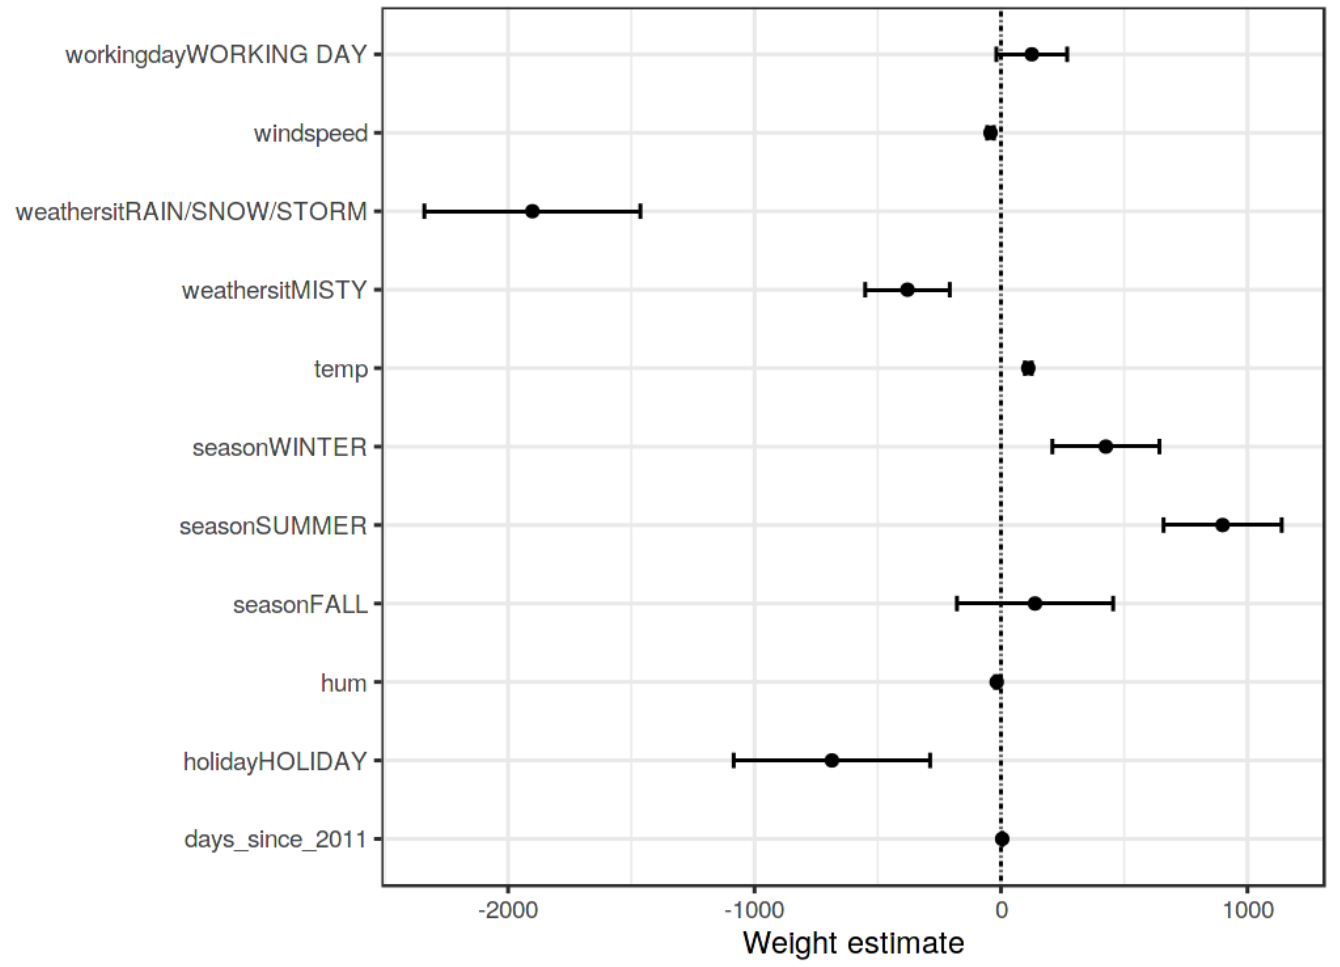
\includegraphics[scale=.2]{images/weight-plot}
		\caption{Weights are displayed as points and the $95\%$ confidence intervals as lines}
		\label{fig:weight-plot}
	\end{figure}
\end{frame}

\begin{frame}{Visual Interpretation: Weight Plot (2/2)}
	\begin{itemize}
		\item<2-> The figure shows that rainy/snowy/stormy weather has a \textbf{strong negative effect} on the predicted number of bikes.
		\item<3-> The weight of the working day feature is close to zero and zero is included in the 95\% interval $\bm{\longrightarrow}$ the effect is \textbf{not} statistically significant.
		\item<4-> Some \textit{confidence intervals} are \textit{very short} and the estimates are \textit{close to zero}, yet the \textit{feature effects were statistically significant} $\bm{\longrightarrow}$ temperature.
		\item<5-> The problem: \underline{the features are measured on different scales}.
		\item<6-> The solution: \textit{scaling the features (zero mean and standard deviation of one) before fitting the linear model}.
	\end{itemize}
\end{frame}

\begin{frame}{Visual Interpretation: Effect Plot (1/3)}
	\begin{itemize}
		\item<2-> The \textbf{weights} of the linear regression model can be more meaningfully analyzed \textit{when they are multiplied by the actual feature values}.
		\item<3-> The \textbf{effect plot} can help you understand how much \textit{the combination of weight and feature contributes to the predictions} in your data.
		\item<4-> The effect of feature $x_j$ for instance $i$ is computed as
		\begin{equation*}
			\onslide<5-> \text{effect}_j^{(i)} = \theta_j \times x_j^{(i)}
		\end{equation*}
		\item<6-> The effects  can be visualized with \textbf{boxplots}.
	\end{itemize}
\end{frame}

\begin{frame}{Visual Interpretation: Effect Plot (2/3)}
	\begin{figure}
		\centering
		\includegraphics<2->[scale=.25]{images/feature-effect-plot}
		\caption{\only<2->{The \textit{feature effect} plot shows the distribution of effects ($= \text{feature value } \times \text{ feature weight}$) across the data per feature}}
	\end{figure}
\end{frame}

\begin{frame}{Visual Interpretation: Effect Plot (3/3)}
	\begin{itemize}
		\item The \textbf{largest contributions} to the expected number of rented bicycles comes from the \onslide<2->{\textbf{temperature feature}} and \onslide<3->{\textbf{the days feature}}, which captures the trend of bike rentals over time.
		
		\bigskip
		\item<4-> \textbf{The temperature} has \textit{a broad range} of how much it contributes to the prediction.
		
		\bigskip
		\item<5-> The \textbf{day trend} feature goes from \textit{zero} to \textit{large positive contributions}, because the first day in the dataset (01.01.2011) has a \textit{very small trend effect} and the estimated weight for this feature is \textit{positive} ($4.93$). \\
		\onslide<6->{This means that the effect $\bm{\uparrow}$ with each day and is \underline{highest} for the \textit{last day} in the dataset (31.12.2012).}	
		\end{itemize}
\end{frame}

\begin{frame}{Explain Individual Predictions (1/4)}
		\onslide<2->{How much has each feature of an instance contributed to the prediction?} \\
		\onslide<3->{This can be answered by computing \underline{the effects for this instance}.} 
	\begin{figure}[!ht]
		\centering
		\includegraphics<4->[scale=.2]{images/the-6th-instance-feature}
		\caption{\only<4->{The 6th instance from the bicycle dataset}}
	\end{figure}
\end{frame}

\begin{frame}{Explain Individual Predictions (2/4)}
	To obtain the feature effects of the 6th instance, we have to \onslide<2->{\textit{multiply its feature values by the corresponding weights} from the linear regression model.} 
	\begin{itemize}
		\item<3-> For the value "WORKING DAY" of feature "workingday", the effect is $124.9$ ($124.9 \times 1$).
		\item<4-> For a temperature of $1.6$ degrees Celcius, the effect is $177.6$ ($1.604356 \times 110.7096$). 
	\end{itemize}
\end{frame}

\begin{frame}{Explain Individual Predictions (3/4)}
	\begin{figure}[!ht]
		\centering
		\includegraphics<2->[scale=.275]{images/effect-plot-6th-instance}
		\caption{\only<2->{The effect plot for the 6-th instance is labeled cross $\times$}}
	\end{figure}
\end{frame}

\begin{frame}{Explain Individual Predictions (4/4)}
	\begin{itemize}
		\item<2-> If we average the predictions for the training data instances, we get an average of $4504$. 
		\item<3-> In comparison, the prediction of the 6th instance is \underline{small}, since only $1571$ bicycle rents are predicted.
		
		\bigskip
		\item<4-> Why?
		\begin{itemize}
			\item<5-> The 6th instance has a \textit{low temperature effect} because on this day the temperature was $2$ degrees, which is low compared to most other days.
			\item<6-> The effect of the \textit{trend feature} "days\_since\_2011" is \underline{small} compared to the other data instances because this instance is from early 2011 ($5$ days) and the \textit{trend feature} also has a \underline{positive} weight.
		\end{itemize}
	\end{itemize}
\end{frame}

\section{Conclusion}
\begin{frame}{Conclusion}
	\begin{itemize}
		\item<2-> We review that a machine learning algorithm can be decomposed into \textit{four components}.
		\item<3-> For the coming future, the focus will be on \textbf{model-agnostic interpretability tools}. \\
		\onslide<4->{Please read \citet{molnar2019}: \emph{Model-Agnostic Methods}.}	 
		\item<5-> Machine Learning will be \textbf{automated} and, with it, \textbf{interpretability}.
		\item<6-> We do not analyze data, we \textbf{analyze models}.
		\item<7-> Robots and programs will explain themselves. For example:
		\begin{itemize}
			\item<8-> A self-driving car that reports why it stopped abruptly ("70\% probability that a kid will cross the road");
			\item<9-> A credit default program that explains to a bank employee why a credit application was rejected ("Applicant has too many credit cards and is employed in an unstable job.");
			\item<10-> A robot arm that explains why it moved the item from the conveyor belt into a trash bin ("The item has a craze at the bottom.")
		\end{itemize}
		\item<11-> Lastly, Interpretability could boost \textbf{machine intelligence research}.
	\end{itemize}
\end{frame}


%\begin{frame}{Machine Learning Model}	
%	\begin{figure}[!ht]
%	\centering
%%	\resizebox{\textwidth}{180pt}{
%	\scalebox{.7}{
%	\begin{tikzpicture}
%%		\draw[help lines] (0,0) grid (15,8);
%		\draw [thick] (0,4) rectangle (3,5.5);
%		\node at (1.5,5) {Features $X$};		
%		\node at (1.5,4.5) {Target $y$};
%		\draw [ultra thick,->] (3.25,4.75) -- (5.25,4.75);
%		\draw [thick] (5.5,4) rectangle (9,5.5);
%		\node at (7.25,5) {Machine Learning};
%		\node at (7.25,4.5) {Algorithm};					
%		\draw [ultra thick,->] (9.25,4.75) -- (11.25,4.75);			
%		\draw [thick] (11.5,4) rectangle (13.5,5.5);
%		\node at (12.5,4.75) {Model};										
%		\draw [ultra thick,->] (12.5,3.75) -- (12.5,1.75);						
%		\draw [thick] (11.5,0) rectangle (13.5,1.5);
%		\node at (12.5,0.75) {$y_{\text{predicted}}$};					
%		\draw [ultra thick,->] (12.5,7.75) -- (12.5,5.75);						
%		\draw [thick] (11.5,8) rectangle (13.5,9.5);
%		\node at (12.5,8.75) {$x_{\text{new}}$};							
%		%\draw (0,3) -- (1.5, 0.5);
%	\end{tikzpicture}
%	}
%	\caption{A machine learning algorithm learns a model from training data.\\ The model is used to make predictions.}
%	\label{fig:machine-learning-model}
%	\end{figure}
%\end{frame}


	

%\section{Survey of major AI application areas}
%\begin{frame}{Computer Vision (1/3)}
%	\begin{itemize}
%		\item Image classification/Object recognition 
%		\begin{center}
%			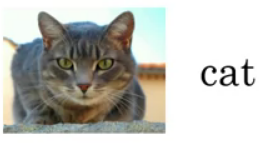
\includegraphics[scale=.4]{images/image-classification}	
%		\end{center}
%		\begin{itemize}
%			\item Face recognition
%			\begin{center}
%				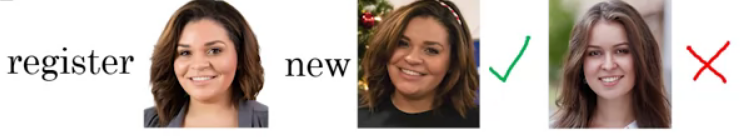
\includegraphics[scale=.35]{images/face-recognition}
%			\end{center}
%		\end{itemize}
%	\end{itemize}
%\end{frame}
%
%\begin{frame}{Computer Vision (2/3)}
%	\begin{itemize}
%		\item Object detection
%		\begin{center}
%			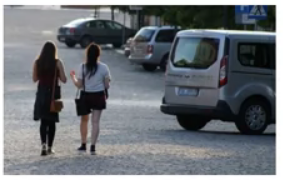
\includegraphics[scale=.4]{images/object-detection-1} \qquad 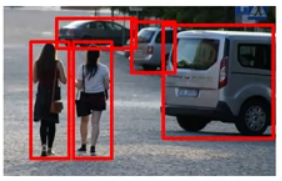
\includegraphics[scale=.4]{images/object-detection-2}
%			\bigskip			
%			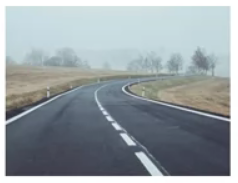
\includegraphics[scale=.4]{images/object-detection-3}	
%		\end{center}
%	\end{itemize}
%\end{frame}
%
%\begin{frame}{Computer Vision (3/3)}
%	\begin{itemize}
%		\item Image Segmentation
%		\begin{center}
%			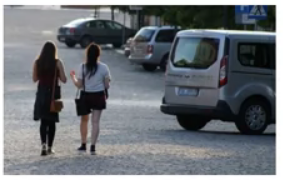
\includegraphics[scale=.4]{images/object-detection-1} \qquad 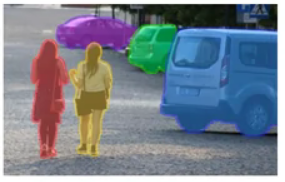
\includegraphics[scale=.4]{images/image-segmentation}	
%		\end{center}
%		\item Tracking
%		\begin{center}
%			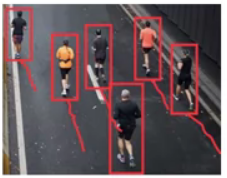
\includegraphics[scale=.4]{images/tracking}
%		\end{center}
%	\end{itemize}
%\end{frame}
%
%\begin{frame}{Natural Language Processing (1/7)}
%	\begin{itemize}
%		\item Text Classification
%		
%		\bigskip		
%		
%		\begin{tabular}{lcl}
%			Email & $\longrightarrow$ & Spam/Non-Spam \\
%			Product description & $\longrightarrow$ & Product category
%		\end{tabular}
%		\begin{itemize}
%			\item Sentiment recognition
%			
%			\begin{tabular}{lcl}
%				"The food was good"     & $\longrightarrow$ & 
\includegraphics[scale=.25]{images/four-stars}	\\
%				"Service was horrible"  & $\longrightarrow$ & 
\includegraphics[scale=.25]{images/one-star}                      
%			\end{tabular}
%		\end{itemize}		
%
%		\bigskip		
%		
%		\item Information retrieval 
%			\begin{itemize}
%				\item E.g., web search
%			\end{itemize}
%	\end{itemize}
%\end{frame}
%
%
%\begin{frame}{Natural Language Processing (2/7)}
%	\begin{itemize}
%		\item Name entity recognition 
%		\begin{center}
%			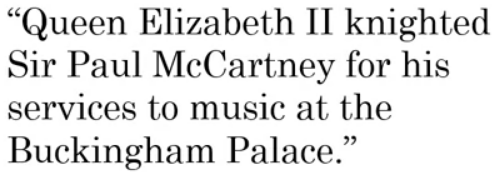
\includegraphics[scale=.25]{images/ner} \qquad 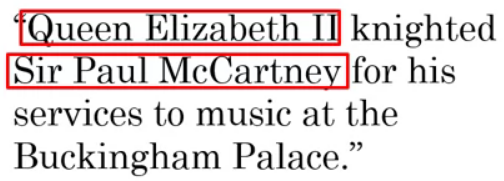
\includegraphics[scale=.25]{images/ner-2} \qquad 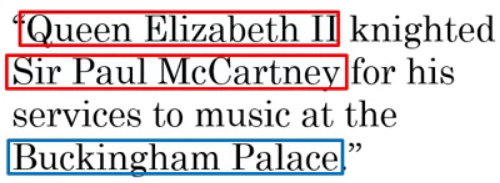
\includegraphics[scale=.25]{images/ner-3}
%		\end{center}
%		\item Machine translation \\
%		"AI adalah listrik baru" $\Longrightarrow$ "AI is new electricity"
%	\end{itemize}
%\end{frame}
%
%\begin{frame}{Natural Language Processing (3/7)}
%	\begin{itemize}
%		\item Others: parsing, part-of-speech tagging
%		\begin{center}
%			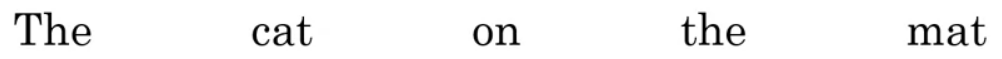
\includegraphics[scale=.25]{images/parsing-1} 	
%		\end{center}
%	\end{itemize}
%\end{frame}
%
%\begin{frame}{Natural Language Processing (4/7)}
%	\begin{itemize}
%		\item Others: parsing, part-of-speech tagging
%		\begin{center}
%			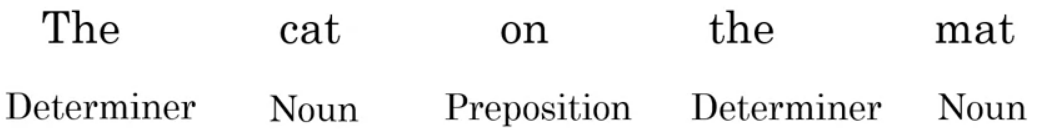
\includegraphics[scale=.25]{images/parsing-2} 	
%		\end{center}
%	\end{itemize}
%\end{frame}
%
%\begin{frame}{Natural Language Processing (5/7)}
%	\begin{itemize}
%		\item Others: parsing, part-of-speech tagging
%		\begin{center}
%			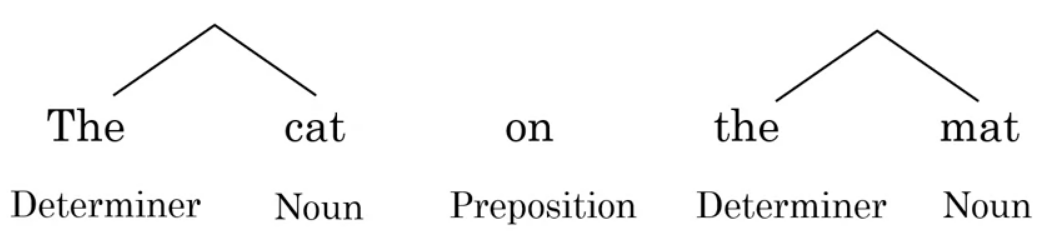
\includegraphics[scale=.25]{images/parsing-3} 	
%		\end{center}
%	\end{itemize}
%\end{frame}
%
%\begin{frame}{Natural Language Processing (6/7)}
%	\begin{itemize}
%		\item Others: parsing, part-of-speech tagging
%		\begin{center}
%			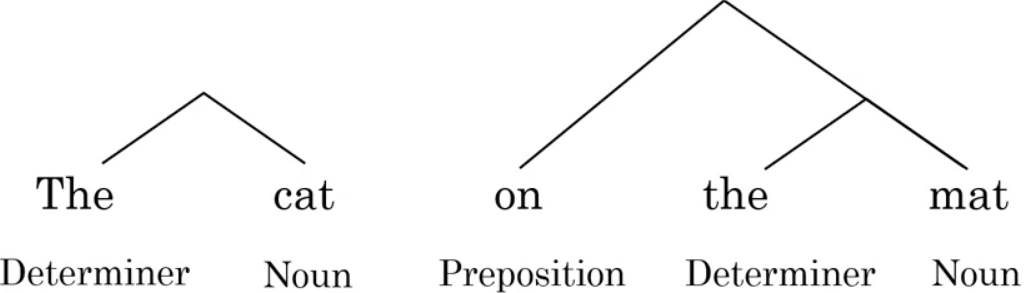
\includegraphics[scale=.25]{images/parsing-4} 	
%		\end{center}
%	\end{itemize}
%\end{frame}
%
%\begin{frame}{Natural Language Processing (7/7)}
%	\begin{itemize}
%		\item Others: parsing, part-of-speech tagging
%		\begin{center}
%			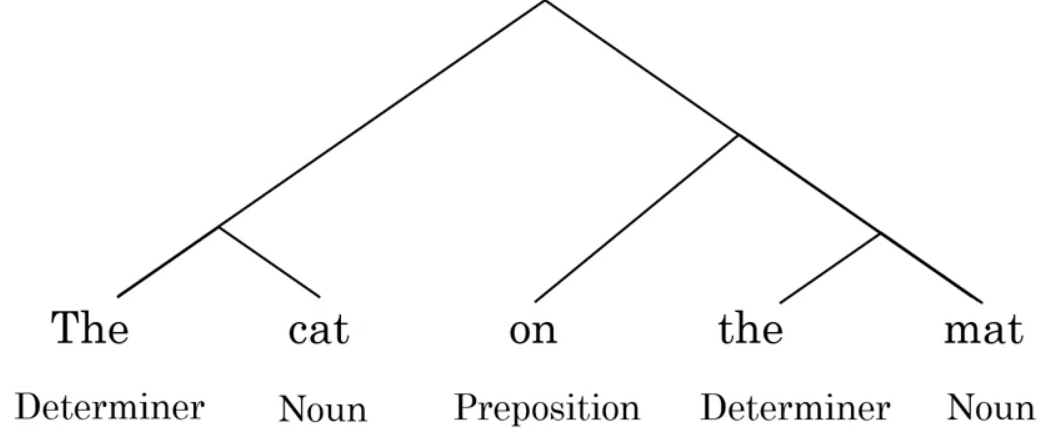
\includegraphics[scale=.25]{images/parsing-5} 	
%		\end{center}
%	\end{itemize}
%\end{frame}
%
%\begin{frame}{Speech (1/2)}
%	\begin{center}
%		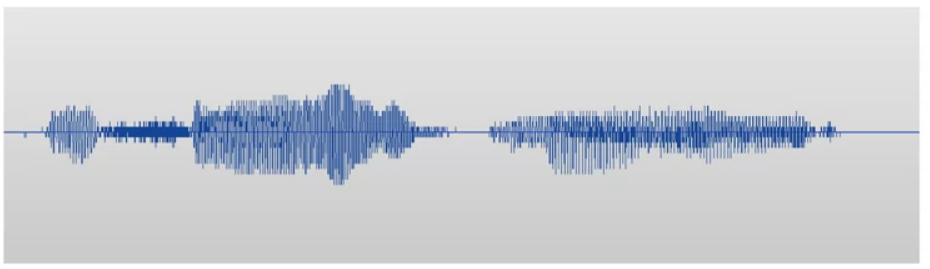
\includegraphics[scale=.25]{images/speech-1}
%	\end{center}
%	\begin{itemize}
%		\item Speech recognition (speech-to-text) \\
%		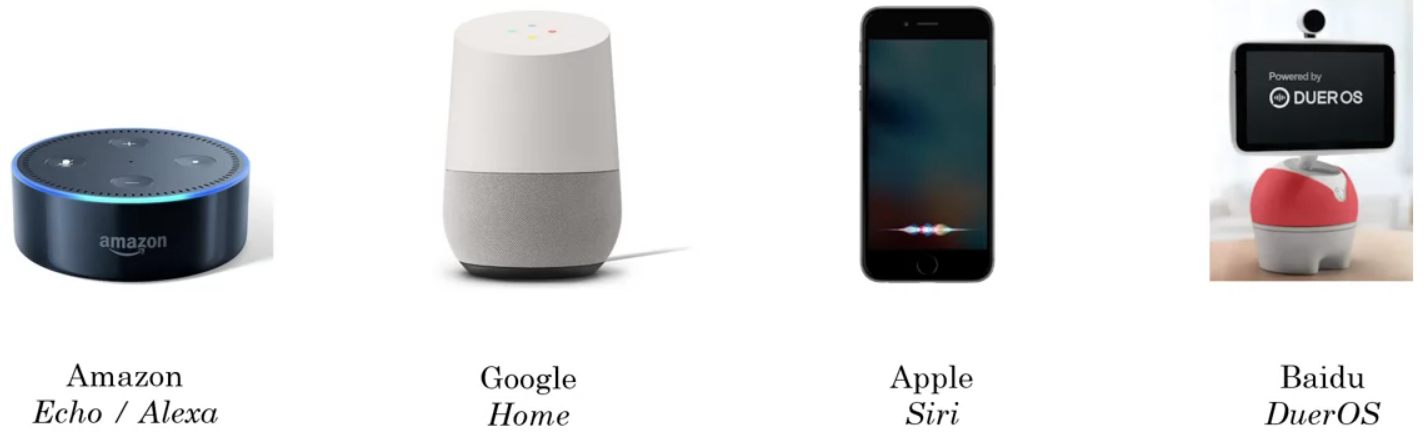
\includegraphics[scale=.2]{images/smart-speakers}
%		\item Trigger word/wakeword detection \\
%		Audio $\longrightarrow$ "Hey device"? (0/1)
%	\end{itemize}
%\end{frame}
%
%\begin{frame}{Speech (2/2)}
%	\begin{itemize}
%		\item Speaker ID
%
%		\bigskip
%
%		\item Speech synthesis (text-to-speech, TTS)
%		\begin{center}
%			\texttt{The quick brown fox jumps over the lazy dog.}	
%		\end{center}						
%	\end{itemize}
%\end{frame}
%
%\begin{frame}{Robotics}
%	\begin{itemize}
%		\item Perception: figuring out what's in the world around you. \\
%		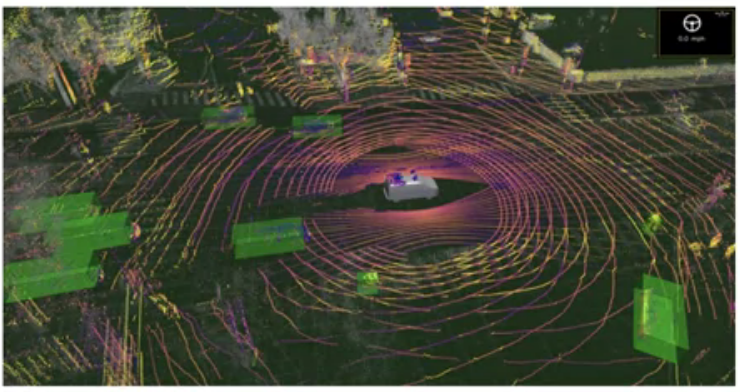
\includegraphics[scale=.2]{images/perception} \; 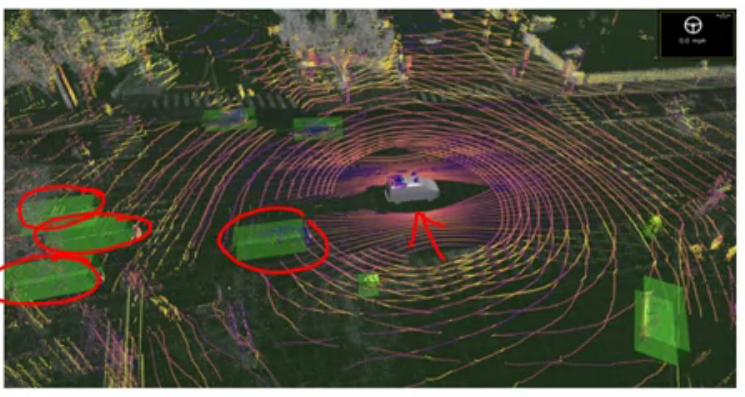
\includegraphics[scale=.2]{images/perception-2} \\
%		\item Motion planning: finding a path for the robot to follow.
%		\begin{center}
%			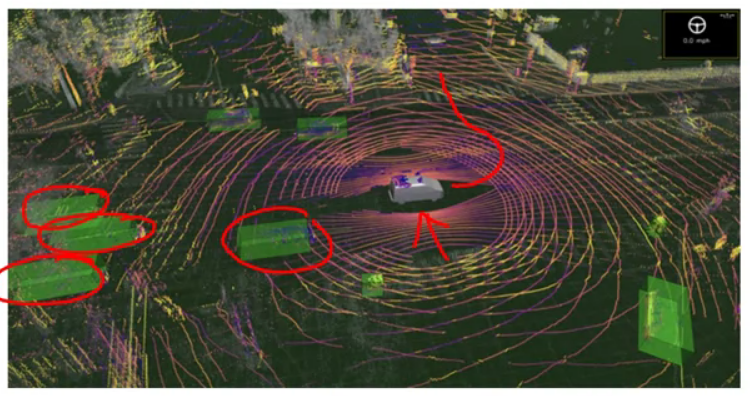
\includegraphics[scale=.25]{images/motion-planning}	
%		\end{center}
%		\item Control: sending commands to the motors to follow a path
%		
%	\end{itemize}
%\end{frame}
%
%\begin{frame}{Unsupervised learning (1/2)}
%	Clustering potato chip sales
%	\begin{center}
%		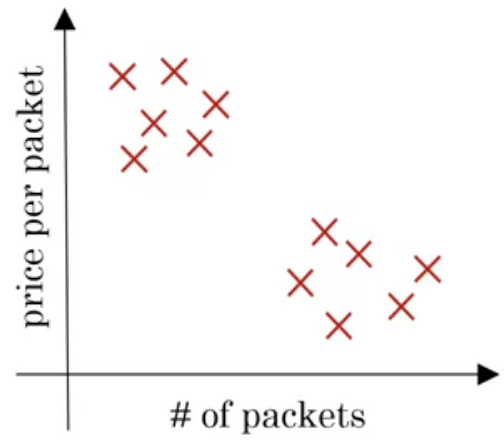
\includegraphics[scale=.25]{images/potato-chip-sales} \qquad 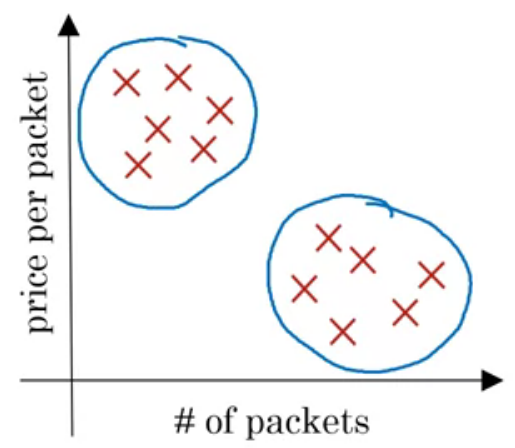
\includegraphics[scale=.25]{images/potato-chip-sales-2}
%	\end{center}
%	
%\end{frame}
%
%\begin{frame}{Unsupervised learning (2/2)}
%	\textbf{Unsupervised learning}:
%	\begin{center}
%		\textit{Given data (without any specific desired output labels), find something interesting about the data.}
%	\end{center}
%	
%	\textbf{Another example of unsupervised learning:}
%	
%	\bigskip	
%	
%	Finding cats from unlabeled YouTube videos
%	\begin{center}
%		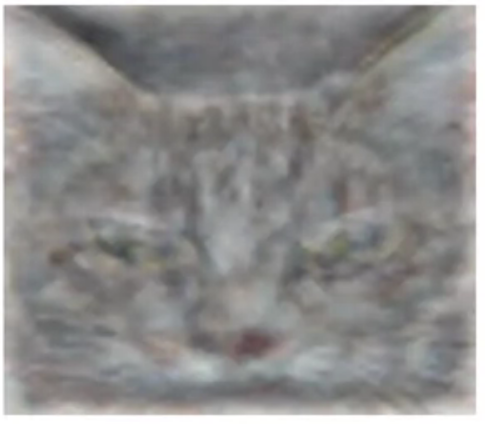
\includegraphics[scale=.25]{images/google-cats}
%	\end{center}	
%\end{frame}
%
%\begin{frame}{Transfer learning}
%	\begin{center}
%		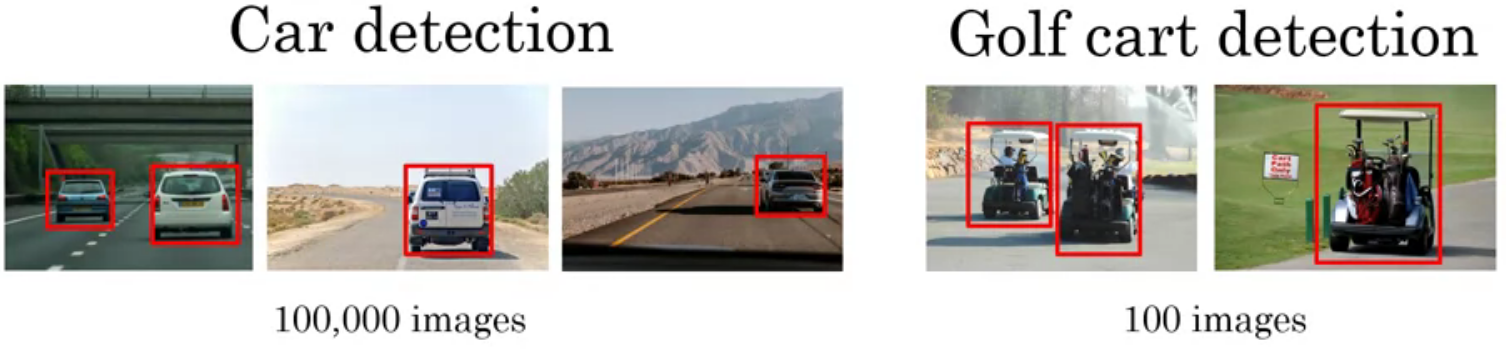
\includegraphics[scale=.225]{images/transfer-learning}
%	\end{center}
%	\begin{center}
%	Learn from task A, and use knowledge to help on task B	
%	\end{center}	
%\end{frame}
%
%\begin{frame}{Reinforcement learning (1/2)}
%	\begin{center}
%		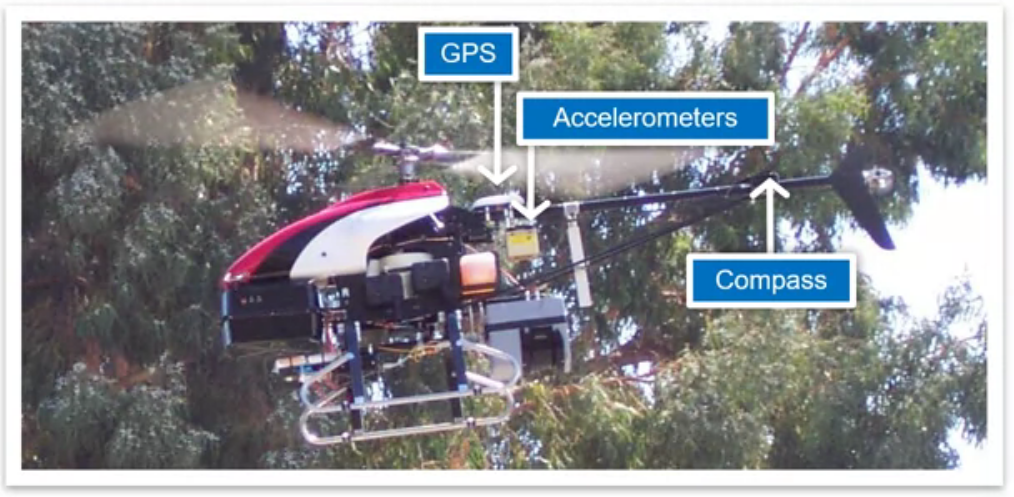
\includegraphics[scale=.325]{images/reinforcement-learning}
%	\end{center}
%	Use a "reward" signal to tell the AI when it is doing well or poorly. It automatically learns to maximize its rewards.
%\end{frame}
%
%\begin{frame}{Reinforcement learning (2/2)}
%	\begin{center}
%		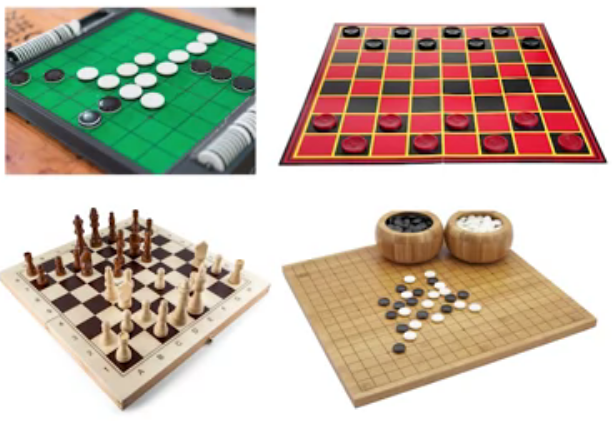
\includegraphics[scale=.325]{images/reinforcement-learning-2}
%	\end{center}
%	Use a "reward" signal to tell the AI when it is doing well or poorly. It automatically learns to maximize its rewards.
%\end{frame}
%
%\begin{frame}{GANs (Generative Adversarial Network)}
%	\begin{center}
%		Synthesize new images from scratch~\citep{karras2017progressive}
%	\end{center}
%	\begin{center}
%		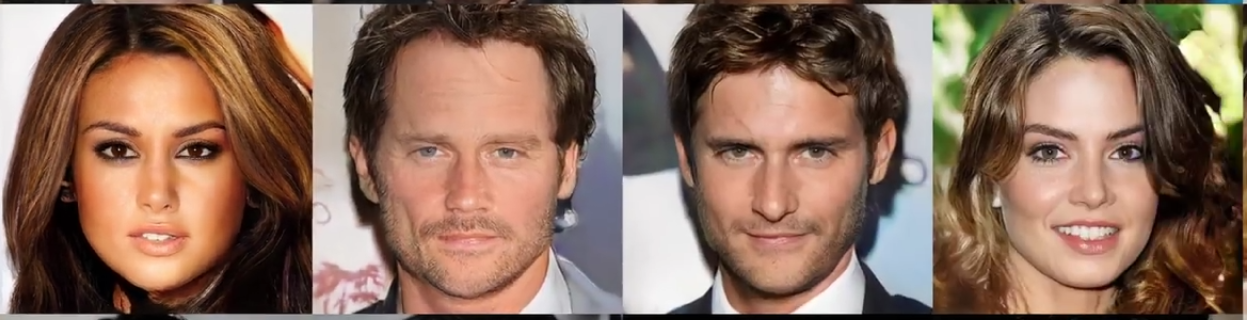
\includegraphics[scale=.25]{images/GANs}
%	\end{center}		
%\end{frame}
%
%\begin{frame}{Knowledge Graph (1/4)}
%	\begin{center}
%		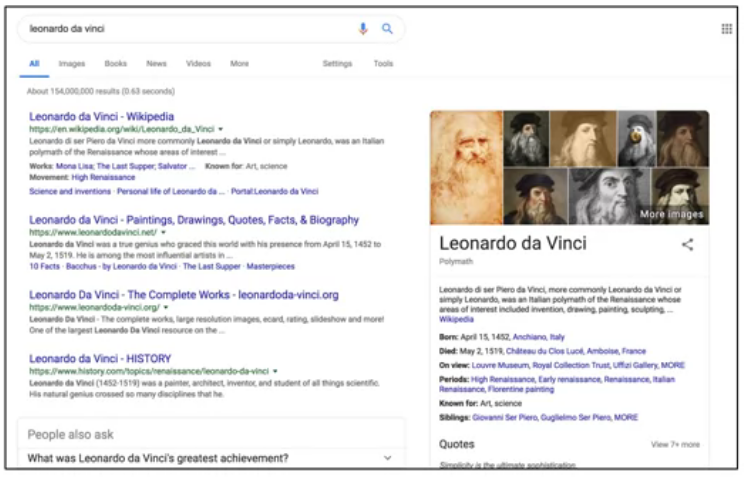
\includegraphics[scale=.35]{images/leonardo-da-vinci}
%	\end{center}
%	
%\end{frame}
%
%\begin{frame}{Knowledge Graph (2/4)}
%	\begin{center}
%		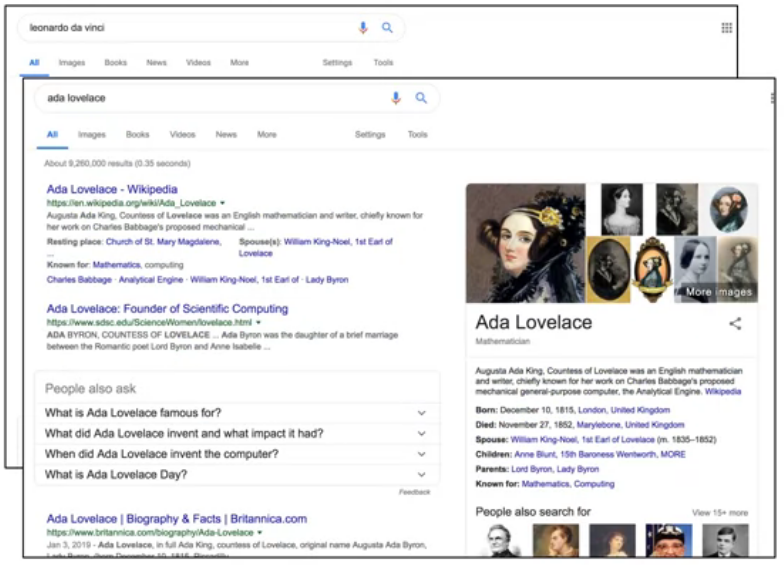
\includegraphics[scale=.35]{images/ada-lovelace}
%	\end{center}	
%\end{frame}
%
%\begin{frame}{Knowledge Graph (3/4)}
%	\begin{center}
%		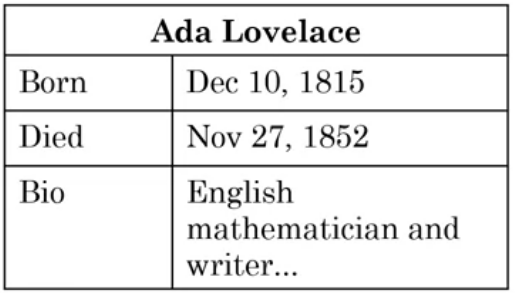
\includegraphics[scale=.35]{images/knowledge-graph-1}
%	\end{center}
%\end{frame}
%
%\begin{frame}{Knowledge Graph (4/4)}
%	\begin{center}
%		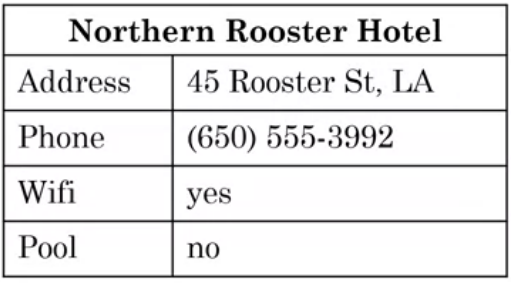
\includegraphics[scale=.35]{images/knowledge-graph-2}
%	\end{center}
%\end{frame}



%\noindent\fbox{%
%    \parbox{\textwidth}{%
%        The quick brown fox jumps right over the lazy dog. 
%    }%
%}











%\begin{frame}{Blocks}
%\begin{block}{Block Title}
%You can also highlight sections of your presentation in a block, with it's own title
%\end{block}
%\begin{theorem}
%There are separate environments for theorems, examples, definitions and proofs.
%\end{theorem}
%\begin{example}
%Here is an example of an example block.
%\end{example}
%\end{frame}


% All of the following is optional and typically not needed. 
\appendix
\section<presentation>*{\appendixname}
\subsection<presentation>*{For Further Reading}

\begin{frame}[allowframebreaks]
  \frametitle<presentation>{Daftar Pustaka}
    {\footnotesize
    \bibliographystyle{apalike}
    \bibliography{references}
    }    
\end{frame}




%\makeatletter % to change template
%    \setbeamertemplate{headline}[default] % not mandatory, but I though it was better to set it blank
%    \def\beamer@entrycode{\vspace*{-\headheight}} % here is the part we are interested in :)
%\makeatother

\begin{frame}[plain]
		\centering
\includegraphics[scale=1]{images/thank-you}	
		hendra.bunyamin@it.maranatha.edu
\end{frame}


%\begin{frame}[plain]
%		\centering
\includegraphics[scale=0.5]{images/Logo-Maranatha-Untuk-Belakang-02}	
%\end{frame}

\end{document}


